\section{Problem 2}

Considering the expression \ref{p2:pavs} for the power available by the source, where $V_S$ is the peak source voltage and $R$ is the source series resistance with the values observed in the figure below we can obtain a power of $P_{av\_s} = \frac{|0.5|^2}{8 \times 50} = 0.625 mW$. The only way to extract all the power from the source is terminating the circuit of the figure below with a load whose resistance matches the source series resistance, in other words a load of $Z_L = 50 \Omega$.

\begin{figure}[H] 
\centering
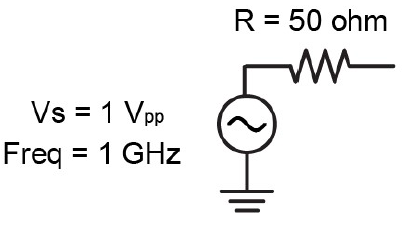
\includegraphics[width=5cm]{images/ckt1p2.png}
\end{figure}

\begin{equation} \label{p2:pavs}
    P_{av\_s} = \frac{|V_S|^2}{8R}
\end{equation}

Despite the previous results, the circuit was terminated with a load of $Z_L = 500 \Omega$ as seen in the circuit of the figure below.

\begin{figure}[H] 
\centering
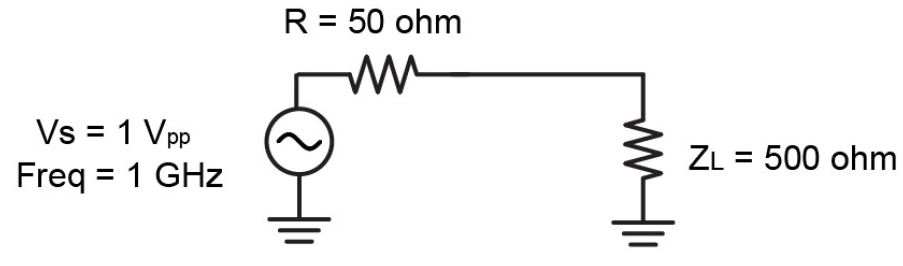
\includegraphics[width=9cm]{images/ckt2p2.png}
\end{figure}

The voltage at the load terminals will obey a simple voltage divider, so that: 

\begin{center}
    $V_L = \frac{Z_L}{R+Z_L} V_S = \frac{500}{50+500}\times 1 = 0.91 V_{pp}$
\end{center}

In this way the power at the load considering the peak voltage is:

\begin{center}
    $P_L = \frac{V_L^2}{Z_L} = \frac{0.455^2}{2 \times 500} = 0.2 mW$
\end{center}

It is clearly seen that the power supplied to the load is way bellow the power available by the source ($P_L < P_{av\_s}$) since there is no match between the source and load impedance. 

An inefficient match can be achieved associating a resistor in parallel with the load to guarantee that the equivalent of the load impedance is $50 \Omega$. The value of the resistor $R_A$ can be founded by the equation below: 

\begin{center}
    $\frac{Z_L R_A}{Z_L+R_A} = 50$
\end{center}

In the way that $R_A = 55.55 \Omega$. Once the match is achieved the load voltage will be $V_L = \frac{V_S}{2} = 0.5 V_{pp}$, but since $R_A<Z_L$, the current flowing through $R_A$ will be higher than the load current and resulting in a loss of efficiency with energy being wasted. This can be shown by the power in each resistor, so that:

\begin{center}
    $P_A = \frac{V_L^2}{2 R_A} = \frac{0.25^2}{2 \times 55.55} = 0.562 mW$ \\ \vspace{10pt}
    and \\ \vspace{10pt}
    $P_L = \frac{V_L^2}{2 Z_L} = \frac{0.25^2}{2 \times 500} = 0.0625 mW$
\end{center} 

Therefore $P_L<P_A$. To confirm that all available power is being extracted from the source, simply add the powers resulting in: $P_L + P_A = 0.562 + 0.0625 \approx 0.625 mW = P_{av\_s}$.

The correct way to ensure the match is with reactive components that, ideally, do not dissipate energy. The circuit of the figure below illustrates the desired matching network.

\begin{figure}[H] 
\centering
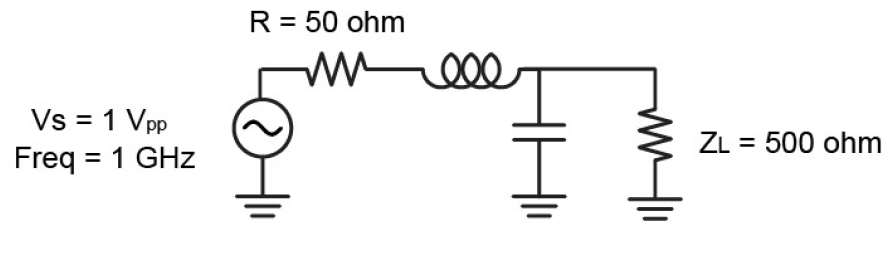
\includegraphics[width=9cm]{images/ckt3p2.png}
\end{figure}

The values of capacitance (C) and inductance (L) can be found via the Smith chart. Resorting to the ADS, the algorithm \ref{p2:alg1} was used to find the values of C and L to guarantee that the normalised impedance ($Z_{eq}$) seen from the source is the real unit (of which correspond to the centre of the chart):
\newline
\begin{algorithm}[H]
\SetAlgoLined
\KwResult{L and C}
 Initialise L and C heuristically\;
 \While{$\Re\{Z_{eq}\} \neq 1$}{
  Keep value of L\;
  Vary the value of C towards $\Re\{Z_{eq}\} = 1$\;
  Find $Z_{eq}$ for the new circuit configuration\;
 }
  \While{$\Im\{Z_{eq}\} \neq 0$}{
  Keep value of C\;
  Vary the value of L towards $\Im\{Z_{eq}\} = 0$\;
  Find $Z_{eq}$ for the new circuit configuration\;
 }
 \caption{How to find the LC impedance matching network via Smith chart}
 \label{p2:alg1}
\end{algorithm}


The algorithm above allowed us to determine a close match with $L=24 nH$ and $C=0.95 pF$, resulting in the Smith chart of the figure \ref{p2:smith1}. Clearly this method does not allow a perfect match since it depends on graphical output, but can be set a admissible error to stop the while loops of the algorithm so convergence is guaranteed.

\begin{figure}[H] 
\centering
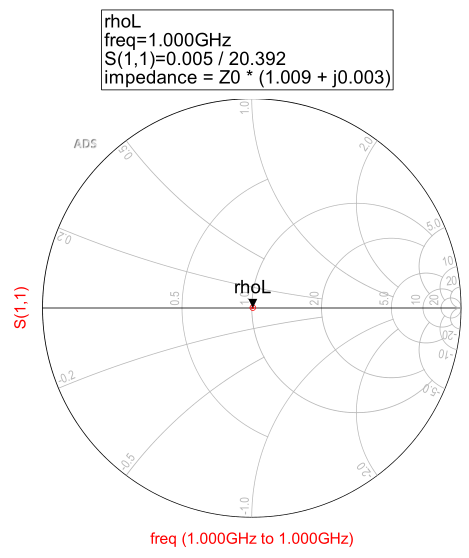
\includegraphics[width=8cm]{images/smith4.png}
\caption{Smith chart for impedance matching in problem 2.}
\label{p2:smith1} 
\end{figure}

Regarding the voltage at the load its value over the transient simulation can be seen in the graph of the figure \ref{p2:plot1} as $V_L = 0.791 V_p$. A curious fact is that the load voltage is higher than the source. This is a direct effect of the matching network that the voltage wave resonates with the natural frequency of the system and provoke a rise in the load voltage. From the source point of view, the load impedance is masked with the same impedance as the source impedance, so even with $Z_L = 500 \Omega$ the load  will extract the total available power because the risen in the voltage will balance the power, so: $P_L = V_L^2/(2 \times Z_L) = (0.791)^2/(2 \times 500) = 0.625mW$

\begin{figure}[H] 
\centering
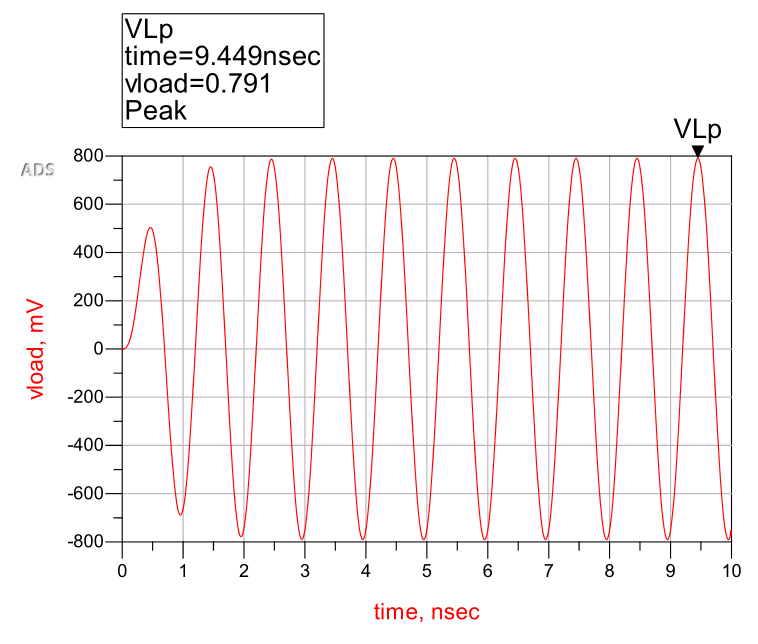
\includegraphics[width=9cm]{images/p2plot1.png}
\caption{Transient simulation of previous circuit with matching network.}
\label{p2:plot1} 
\end{figure}
